\documentclass{article}
\usepackage[margin=1.0in]{geometry}
\usepackage{setspace}
\usepackage{graphicx} % Required for inserting images
\usepackage{xcolor}
\usepackage{amsmath}
\usepackage{amssymb}

\onehalfspacing

\title{Understanding the Cost of School Lottery Participation}
\author{Kyle Woodward and ???}
\date{December 2025}

\begin{document}

\maketitle

\section{Introduction}
In the 2023--2024 school year, the San Francisco Unified School District (SFUSD) announced that SFUSD transitional kindergarten (TK) students would qualify for automatic promotion to their TK's associated elementary school, allowing families to bypass SFUSD's kindergarten lottery process. Families of 2024--2025 TK students were therefore the first to feasibly "opt out" of SFUSD's application lottery (specifically, the lottery for 2025--2026 kindergarten seats).

At a high level, these families clearly chose to opt out. In a typical year, roughly 4000 kindergarten families apply for seats in SFUSD. During the 2025--2026 application cycle, roughly 600 of 800 eligible families (just under 75\%) chose automatic promotion into their TK's associated kindergarten program. This 15\% (600 out of 4000) drop in lottery participation corresponded almost exactly to a 15\% drop in ranked seat applications (from 22600 to 19300). This suggests that the families who accepted automatic promotion are, in some sense, representative of lottery participation on the whole and are not, for example, particularly disposed to rank more or fewer seats than average.

A notable feature of SFUSD's TK program is that it is intentionally designed to drive prospective students to under-demanded schools (ed. this is gossip/grapevine). Under the assumption that families place greater value on over-demanded schools (hence their excess demand), when families accept the opt-out offer they (on average) trade a relatively high-payoff, uncertain outcome for a relatively low-payoff, certain outcome. Popular discourse regarding SFUSD's lottery---and school lotteries in general---indicates that families are displeased with the uncertain nature of lottery outcomes. SFUSD's TK opt-out policy allows us to measure the precise extent of this unhappiness: look at where the families who opted out could have gone, then compare their expected payoff from lottery participation to their realized payoff from opting out of the lottery. The difference is their distaste for lottery participation.

(lots of discussion about selection)

Previous work has provided dollar-denominated estimates for families' value for school quality (cf. ...). This is possible because certain aspects of school preferences---e.g., commute distance---are roughly convertible to money, hence all preference terms may be measured in this unit. Our results on the "preference" cost of lottery participation therefore have a simple interpretation: how much do families need to be compensated to participate in SFUSD's lottery. This suggests a natural policy prescription: to encourage lottery participation, SFUSD should offer a simple \$xxx benefit to families who participate.

(discussion about SFUSD's relationship to private schools)


\section{Model}
We apply a standard logit model of school preferences. Thus the number of schools a family applies to is a function of a (time-varying) outside option.

(in reality, school qualities are family information are also time-varying, but we don't have that data right now)

(write out preference specification)

(we also just did some dumb regressions, but it will be helpful to think structurally)

Taken this way, the number of applications to a school is the total number of students applying in this cycle, times the year-dependent probability that the school is better than the outside option,
\[
A_{kt} = N_t \times \Pr\left( \theta_k\geq \theta_{0t} \right) \;\; \implies \;\; \ln A_{kt} = \ln N_t + \ln \theta_k - \ln \left[ \exp \theta_k + \exp \theta_{0t} \right].
\]
Standard identification arguments give
\[
\ln A_{kt} - \ln\left[ N_t - A_{kt} \right] = \ln \theta_k - \ln \theta_{0t}.
\]

\textbf{Observation.} The number of applications $N_t$ is endogenous to the quality of the outside option $\theta_{0t}$. However, we note that the average applicant applies to 5 schools; IIA in the logit model implies that, empirically, $N_t$ should be effectively independent of $\theta_{0t}$.

(these results are similar to those for the model where the application probability is fixed; but there is not a micro-model for this that is consistent with time-varying total rank volume)

Now that we actually plot it, TK-promotion eligibility appears roughly unrelated to measured school quality.
\begin{figure}
    \centering
    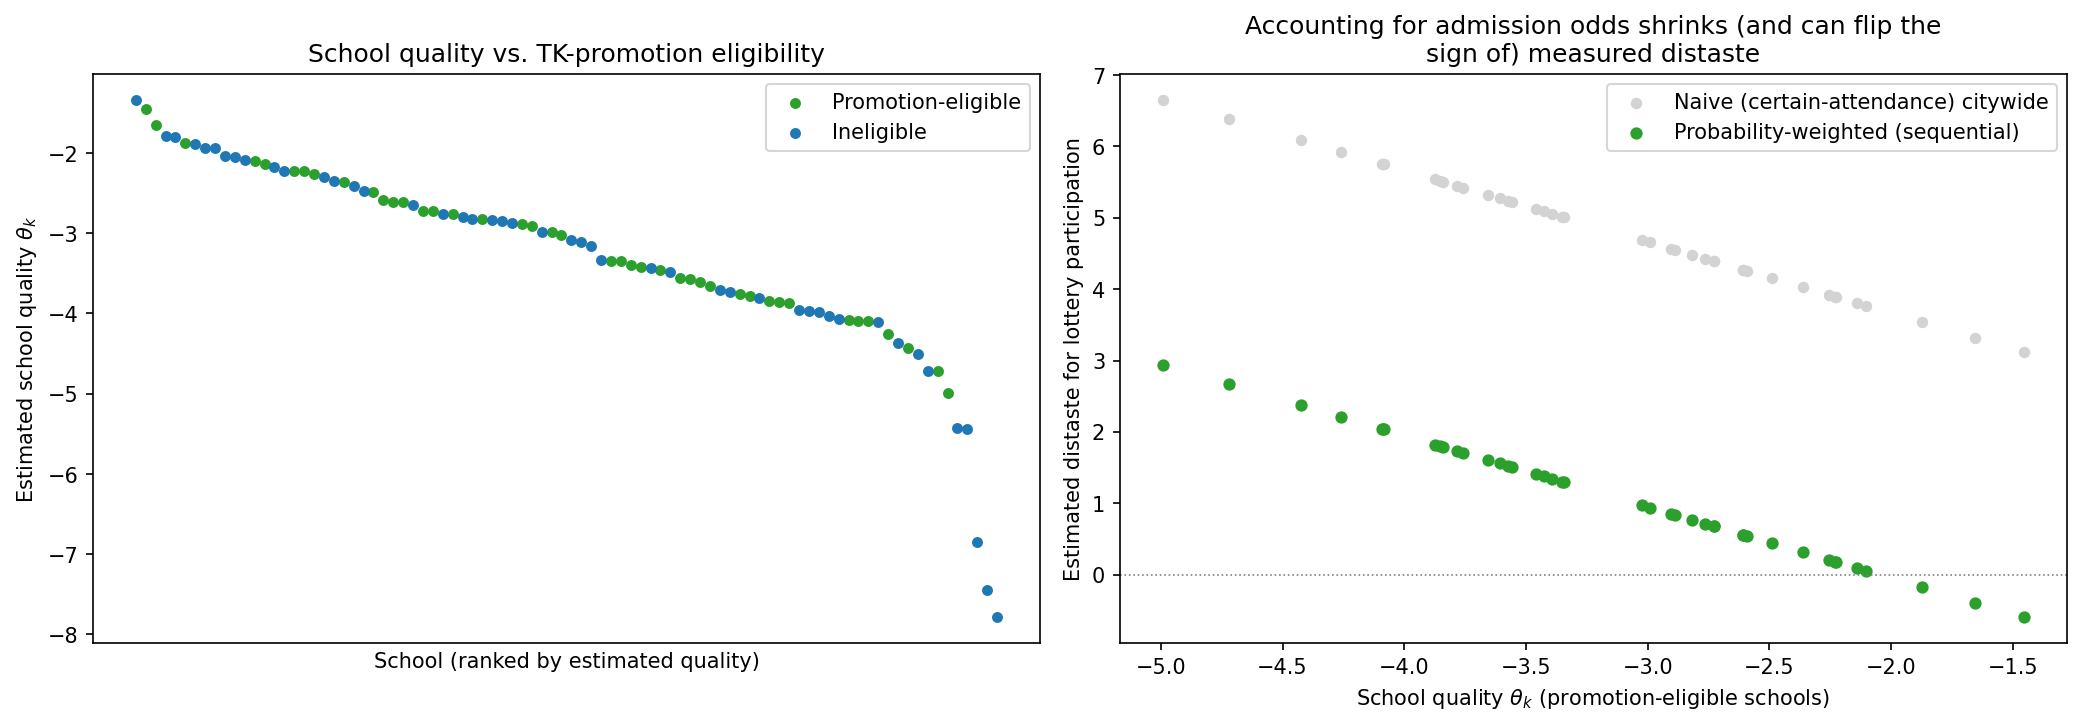
\includegraphics[width=\linewidth]{figures/quality_by_promotion_status.png}
    \caption{Left: estimated school quality $\theta_k$ (school fixed effect from the log-request-share regression), all K schools ranked by quality, colored by TK-promotion eligibility. Promotion-eligible schools are spread across the quality distribution rather than concentrated at either end, though they are somewhat overrepresented in the lowest tail, consistent with the (informal) claim that TK placements skew toward under-demanded schools. Right: the citywide-inclusive-value distaste measure (\S\ref{sec:cost-of-application}) plotted against $\theta_k$ for promotion-eligible schools only.}
    \label{fig:quality-by-promotion-status}
\end{figure}

write out the formula for substitution

Automatic promotion reduces the number of applicants for the 2025--2026 school year by precisely the number of students who accept automatic promotion. We observe 3380 students applying for seats via the lottery, while 601 accept automatic promotion. It follows that automatic promotion reduces applications to schools not associated with TK programs by 15.1\%.

On the other hand, we observe the number of students who accept automatic promotion at all schools associated with TK programs. Letting $P_{tk}$ be number of students who accept automatic promotion in year $t$ at school $k$, and $P_t = \sum_k P_{tk}$, the impact of automatic promotion is
\[
\left[ N_t \times \Pr \left( \theta_k \geq \theta_{0t} \right) + P_{tk} \right] - \left(N_t + P_t \right) \times \Pr\left( \theta_{k} \geq \theta_{0t} \right).
\]
In relative terms, this is
\[
\frac{P_{tk}}{\left( N_t + P_t \right) \times \Pr\left( \theta_k \geq \theta_{0t} \right)} -\frac{P_t}{N_t+P_t} = \frac{1}{N_t + P_t} \left[ \frac{\exp\left( \theta_k \right) + \exp\left( \theta_{0t} \right)}{\exp\left( \theta_k \right)} P_{tk} - P_t \right].
\]
The mean impact at promotion-eligible schools is 13.8\%. These schools also saw a decrease, because even though they are guaranteed "applications" there is a large body of students who would otherwise possibly apply to their program.]

Now we take this to a structural model of why people don't apply to schools. This is an expected value calculation based on estimated $\theta_k$ values.

\subsection{The cost of application}
\label{sec:cost-of-application}
Observe that our quality estimates $\theta_k$ are estimates of the value of application, not attendance. Thus to understand the cost of lottery participation, we need to adjust qualities for the probability of attendance. That is, a family that chooses automatic promotion is for-sure attending that school, hence their probability of attendance is $1$, in general strictly larger than the probability of attending that school via the lottery process.

\begin{itemize}
    \item We can create probability-unweighted quality scores; this is the easiest approach
    \item We could also take note of the fact that some families choose to enter the lottery anyway. This is either evidence of heterogeneous quality learning, or of a hierarchical logit approach.k
\end{itemize}

\paragraph{A first (probability-unweighted) estimate.} Taking the easy approach above, a family offered automatic promotion into school $k$ trades the certain, unweighted payoff $\theta_k$ for the uncertain payoff of remaining in the lottery. Under the logit model, the expected payoff of facing a choice set $S$ under i.i.d.\ Type-I extreme value shocks is its inclusive value $\ln \sum_{j \in S} \exp(\theta_j)$, so the option value a family gives up by accepting promotion---their distaste for lottery participation---is
\[
\text{distaste}_k = \ln \sum_{j \in S} \exp(\theta_j) \; - \; \theta_k .
\]
We compute this two ways, differing only in $S$:
\begin{itemize}
    \item \emph{Citywide}: $S$ is every K school in the panel (86 schools). This is the more informative number---roughly, how much better is the best school a family could plausibly have won---but it has a much sharper problem than geographic scope: the inclusive-value formula implicitly assumes a family can costlessly \emph{attend} whichever school in $S$ they'd prefer, i.e.\ that choice probability equals attendance probability. That's exactly the assumption this section opened by flagging as wrong---application counts (and hence $\theta_k$) say nothing about the odds of actually being assigned a seat once a family applies, and those odds are certainly $<1$ at oversubscribed schools. Left unweighted, the citywide measure is therefore a substantial overstatement, not just a mild one: see the numerical check below.
    \item \emph{Binary}: $S = \{k, \text{outside option}\}$, matching the paper's own two-alternative identification above, with the outside-option level $\theta_{0t}$ recovered from the fitted application-year fixed effect. Because any single school is a small share of citywide demand, $\theta_{0t}$ sits close to its normalized zero point in every year, so this measure is close to degenerate: it collapses to approximately $-\theta_k$ and adds little beyond the raw quality estimate. We report it mainly as a conservative check on the citywide number.
\end{itemize}
Averaging across the 601 families who accepted automatic promotion for 2025--2026 (weighting each promotion-eligible school by how many of its families opted out), the citywide measure gives a mean distaste of $4.78$ log-utility units, versus $3.08$ under the (degenerate) binary measure. Figure~\ref{fig:quality-by-promotion-status} (right panel) shows this distaste measure is, mechanically, close to linearly decreasing in $\theta_k$: families zoned to already-low-demand TK schools are estimated to give up more by accepting promotion than families zoned to comparatively higher-demand TK schools.

\paragraph{How big is $4.78$, really?} Log-utility units aren't interpretable on their own, so it helps to translate the gap into real schools. A distaste of $4.78$ is about the same size as the $\theta$-gap between Clarendon ES ($\theta=-1.32$, the single best K school in the district by this measure) and Havard Tk ($\theta=-5.44$, ranked 83rd of 86)---i.e.\ nearly the \emph{entire} citywide quality range. For context, the full range spanned by the 42 promotion-eligible schools themselves, best to worst, is only $3.61$: smaller than the citywide distaste figure. This is a direct, visible symptom of the attendance-probability problem raised above: the citywide inclusive value itself is $1.67$, which exceeds even Clarendon's raw $\theta$ of $-1.32$---the model is crediting families with an expected payoff better than the best real seat in the district, only possible because it assumes they can have whichever school they want with certainty. A properly probability-weighted version would require joining seat-capacity data (by school, grade, and year) against request volume to construct real admission-probability weights; that data isn't joined into this pipeline yet, so both numbers above should be read as upper bounds, and the citywide one is the less trustworthy of the two precisely because it lets a family "choose" across a far larger set with no risk penalty. Per-school comparisons for both measures are in the \texttt{\_comparable\_to} columns of \texttt{output/lottery\_distaste\_estimates.csv}.

These numbers are in log-utility units, not dollars---we don't yet have a commute-cost-based (or other) utility-to-dollar conversion joined into this pipeline, so the policy-relevant \$xxx figure floated in the introduction is still future work.

\paragraph{A probability-weighted estimate.} The unweighted approach above also leaves the second bullet unaddressed: roughly a quarter of eligible families entered the lottery anyway despite being offered a certain seat, which a model with strictly non-negative option value for every family cannot rationalize. Both problems trace to the same source, so we fix them together by actually weighting for probability of attendance.

A family that ranks schools by preference and is assigned the highest-ranked school that admits it has expected payoff
\[
\mathbb{E}[U] = \sum_{k=1}^{K} \theta_k \, P_k \prod_{j \prec k} \left( 1 - P_j \right),
\]
where schools are indexed $1, \dots, K$ in decreasing order of $\theta$ (truthful preference order, given SFUSD's mechanism is strategy-proof), $j \prec k$ denotes every school ranked above $k$, and $P_k$ is school $k$'s admission probability. This is exactly $P(\text{admit}_1)\theta_1 + P(\text{admit}_2)P(\text{reject}_1)\theta_2 + \cdots$: a family only reaches its $k$-th choice if it was rejected everywhere it ranked higher. We treat rejection as independent across schools---a simplification forced by not observing individual-level match outcomes, which would let rejections correlate (e.g.\ through a common lottery number) in ways we cannot identify here.

$P_k$ itself we proxy with $\min(1, \text{capacity}_k / \text{demand}_k)$: $\text{demand}_k$ is school $k$'s average total (all-rank) lottery request volume across the panel, and $\text{capacity}_k$ is its actual kindergarten enrollment, averaged over the two most recent CDE school-level enrollment files (2023--24, 2024--25)---occupied seats being the closest available proxy for how many seats exist. Matching lottery school names to CDE school names by hand for the 71 (of 86) schools with a confident match gives admission probabilities from $4.5\%$ (Clarendon ES, the single most oversubscribed school) up to real capacity-constrained rates in the teens and twenties for less-demanded schools---all economically sensible, and a sharp departure from the unweighted approach's implicit $P_k=1$. The remaining 15 schools are standalone TK program sites with no separately reported kindergarten enrollment (either co-located without their own CDS code, or reported as TK/pre-K-only "Children Centers"); rather than risk wrongly assigning them a same-named elementary building's capacity, we exclude them from matching and fall back to $P_k=1$, which is also the least distortive default available given that these are, by construction, the lowest-$\theta$ schools in the panel. Code and the full crosswalk are in \texttt{src/capacity.py}.

Plugging in gives a citywide $\mathbb{E}[U] = -2.02$---below Clarendon's raw $\theta$ of $-1.32$, as it must be once admission is genuinely uncertain, unlike the naive citywide inclusive value ($1.67$) computed above. The resulting distaste measure, $\text{distaste}^w_k = \mathbb{E}[U] - \theta_k$, averages $1.08$ across the 601 families who accepted automatic promotion (family-weighted)---about a \emph{quarter} of the naive citywide estimate ($4.78$) and a third of the binary one ($3.08$). Translated into real schools again: $1.08$ is comparable to the $\theta$-gap between Clarendon ES and Monroe ES (\#23 of 86), a far more plausible "typical foregone opportunity" than nearly spanning the entire district.

Crucially, three schools---West Portal ES, Alvarado ES, and Rooftop K-8, all among the highest-$\theta$ (least under-demanded) TK-linked schools---now have \emph{negative} probability-weighted distaste: our model says a family zoned there is better off taking the certain seat than gambling on the lottery, admission odds included. This partially answers the puzzle above: families zoned to these three schools who nonetheless entered the lottery were, by this model, taking a negative-expected-value bet (heterogeneous beliefs, a genuine idiosyncratic draw realization we don't observe, or simply a model misspecification are all still on the table---but at least the model no longer rules out a rational family ever preferring to skip the lottery). Figure~\ref{fig:quality-by-promotion-status} (right panel) plots both measures side by side; per-school detail, admission probabilities, and the full CDE-matching crosswalk are in \texttt{output/lottery\_distaste\_estimates.csv} and \texttt{output/school\_admission\_probabilities.csv}.

This is still not the dollar-denominated answer the introduction wants, and the independence assumption above is a real one (true deferred-acceptance rejections likely correlate through priorities and lottery numbers in ways that would push $\mathbb{E}[U]$ further down, since correlated rejection reduces the value of a long list relative to independent draws). But it is a substantively different, more credible number than either unweighted measure, and it directly operationalizes the adjustment this section originally set out to make.

The full per-school results are in \texttt{output/lottery\_distaste\_estimates.csv}; \texttt{output/lottery\_distaste\_summary.csv} carries the family-weighted and unweighted means above, and the estimation code lives in \texttt{run\_distaste\_analysis.py} and \texttt{src/}.

\section{Other concerns}
\begin{itemize}
\item Learning (by being at the school)
\item Endowment effect
\item Selection (people who know they want to go to the school)
\item The fact that, implicitly, measured preferences based on rank applications are net of acceptance probability
\end{itemize}
\end{document}
